% This example An LaTeX document showing how to use the l3proj class to
% write your report. Use pdflatex and bibtex to process the file, creating 
% a PDF file as output (there is no need to use dvips when using pdflatex).
% Modified 

% This dissertation was built upon base template provided.

\documentclass{l3proj}

\begin{document}

\title{Team I: ResDiary Restaurant Recommendation System}

\author{Vladimir Bardarski \\
        Paulius Dilkas \\
        Domantas Jurkus \\
        Edward Kalfov \\
        Josh O'brien \\
		Joseph O'Hagan}

\date{31st March 2017}

\maketitle

% ##################################################
% LAST EDIT: 	06/03/17	Joseph
% ##################################################
\begin{abstract}
The abstract shall go here! Here is some things to keep in mind while writing it.
\end{abstract}

\begin{itemize}
\item The abstract is likely the first substantive description of your work read by an examiner. View it as an opportunity to set accurate expectations.
\item The abstract is a summary of the whole thesis. It presents all the major elements of your work in a highly condensed form. (Write it having written the rest of the paper) The paper sets the abstract.
\item It must be capable of substituting for the whole paper when there is insufficient time and space for the full text.
\item Keep it short and snappy. 
\item The primary function of your thesis (and by extension your abstract) is not to tell readers what you did, it is to tell them what you discovered.
\item Approximately the last half of the abstract should be dedicated to summarizing and interpreting your results.
\item The most common error in abstracts is failure to present results.
\end{itemize}

% Comment out this line if you do not wish to give consent for your work to be distributed in electronic format.
% We hereby give consent - spread the knowledge - pending on result of project
\educationalconsent

\newpage

%==============================================================================

% ##################################################
% LAST EDIT: 	06/03/17	Josh
% ##################################################
\section{Introduction}
% An introduction, explaining the purpose of the document, a very brief outline of the project and a summary of the structure of the rest of the document (approximately 1-2 pages).

The Professional Software Development (PSD3) course at The University of Glasgow requires students to engage with the practices and methodologies used in modern large-scale software engineering. The purpose of this dissertation is to document the development of the software project created as part of this course by Team I. 

The project was to build, over the course of several months, a restaurant recommendation engine for the Glasgow-based company ResDiary.
The goal was to deliver a system which could produce recommendations for restaurants to a user, that could be integrated into their existing systems at a later date. 
% Do we delay mentioning the integration at this stage? - Joseph?
% Do we make it clear here it was recommendations based on similar users? - Joseph?

Our team consisted of six third-year Computing Science students. Within the group there was a broad array of skills, interests and experience - with two members actively working as software professionals, and another having participated in an internship. For some members, however, this was a first opportunity to interact with a real client. 

In this document we outline, in detail, the entire process: from the initial requirements gathering with our customer, through to final system delivery. 

In section \ref{sec:background} we present the background to the project, the motivations of the customer and how we arrived at the agreed deliverables.

%this will surely be expanded to enumerate each separate section better I would like to discuss in detail the practices, issue-tracking, the team work/team load - Josh etc.

In subsequent sections \ref{sec:alice} through Section \ref{sec:reflections} we explore the challenges we faced through development and the steps we took to resolve them, explore the impact of team dynamics on the outcome and reflect on what we have learned from the experience. We also explain how we applied the good development practices learned in PSD3. In particular we highlight the role of version control, agile development and issue tracking.

\newpage

%==============================================================================

\section{Case Study Background}
\label{sec:background}
% A description of the case study background and context. This should include a description of the project customer (what was the nature of the organisation you were working for), their objectives for the project, and a summary of what was actually achieved. Where appropriate, this section should also make reference to similar related projects in order to make the context clear (approximately 4-5 pages).

% MISC POINTS TO DISCUSS:
% 1. Do we address the legal contract we signed. I.e. Initially it was proposed for integration into the site. It then changed and this we reflected in the contract we signed which outlined the final product and how it could be used be ResDiary - possibly get a more accurate summary of what ResDiary can do with the delivered product from them (ask them to summarise the contract essentially mentioning it is beneficial to our final report)

% ##################################################
% LAST EDIT: 	06/03/17	Joseph
% ##################################################
\subsection{Customer}
\label{customer}
% The customer organisation and background.

% Here we want answer the question of who are ResDiary and what do they do.
% Additionally answer who played the customer role of ResDiary to us on the project.


% Who are ResDiary?
ResDiary are a Glasgow-based online restruant reservation founded in 2006. They are a commerical organisation whose service provides a comprehensive and easy to use booking platform and table management system that is used by both the hospitality industry and its guests. The service provides 24-hour reservation services via customer websites such as Facebook and Twitter. Their global service sees 9.7 million covers booked every month and their technology is in use in over 6,500 restaurants across 58 countries.

For the duration of the project ResDiary senior software engineers Adam Connelly and Ian Strachan acted as the representatives of ResDairy. They served as the point of contact between our team and the customer and provided useful feedback and answers to our queries throughout the development of the project. They also provided supplies of data for use within the project upon request with steps taken by ResDairy to ensure anonaminity of the sensitive user data.


% ##################################################
% LAST EDIT: 	06/03/17	Joseph
% ##################################################
\subsection{Initial Objectives And Rationale}
\label{initobjectives}
% The rationale and initial objectives for the project.

% Essentially with the intro we want to introduce the company and the aims of the project. Mention similar real world examples such as the Netflix model as this was used as a reference / example similar project early on in our project. Talk out the specification, reference the dropped features of the specification in relation to what was actually developed and presented to the customer. Potentially mention points of future expansion as well and how project was setup to account for those future developments.

% Possibly reflect on the change in specification that occurred - how it was originally proposed to what it evenually became both from our perspective (in terms of what we would develop) and how ResDiary wished to use the project (in that they intially proposed either integrating it into their system or creating an API to eventually just wanting it as a proof of concept to learn from).

% Essentially I want to introduce the customer and provide an overview of the motivation of the project.
% Project motivation comes from three reasons:
% 	1. Improve restaurant discover on existing service 
%	2. Commerial reason as it is not something their competition does
%	3. Big data proof of concept research - they have large amount of big data they do nothing with and would like to see if using it for such a purpose would be useful

% This is rough but I'm trying to mainly hit on the motives and tease on some later developments


% Initial Meeting - Project Motivation - Initial Aims
Our initial meeting with the customer was led by Ian Strachan and served as the customer requirements elicitation meeting. The meeting began with an overview of the ResDairy business (link to customer section) and the technologies currently in place. One shortcoming of their existing systems however is that the large quantity of big data gathered by ResDiary in their day-to-day operations is currently unused and dorminant. 

A proposed method (and our project) for utilising this data is to improve restaurant discovery of the ResDairy portal (found at ResDiary.com) by implementing a recommendation system into the service. They wished for recommendations to be made to suggest restaurants to a user based off other users with similar dining habits. They believed such a system would distinguish them from their competition as their research shows it is not a feature in place by their competition. Similar systems referenced in existing services include the Netflix model and Amazon model for making recommendations to users (reference via papers here). Hence our project was to create a restraunt recommendation system for ResDairy and should time allow it potentially integrate it into their existing service. This final goal would later change over the course of development (reference change around iteration 3 for project goal) as ResDiary wished to use the project to act as a proof of concept which they could use to assess its quality and usefulness to them and whether integration of a similar system into their own site would be beneficial.


% ##################################################
% LAST EDIT: 	06/03/17	Joseph
% ##################################################
\subsection{Delivered Software}
\label{finsoftware}
% Information on the final software that was delivered to the customer.

\newpage

%==============================================================================
\section{Alice}
\label{sec:alice}

This is a example of how to include an image from the figures directory.

\begin{figure}
\begin{center}
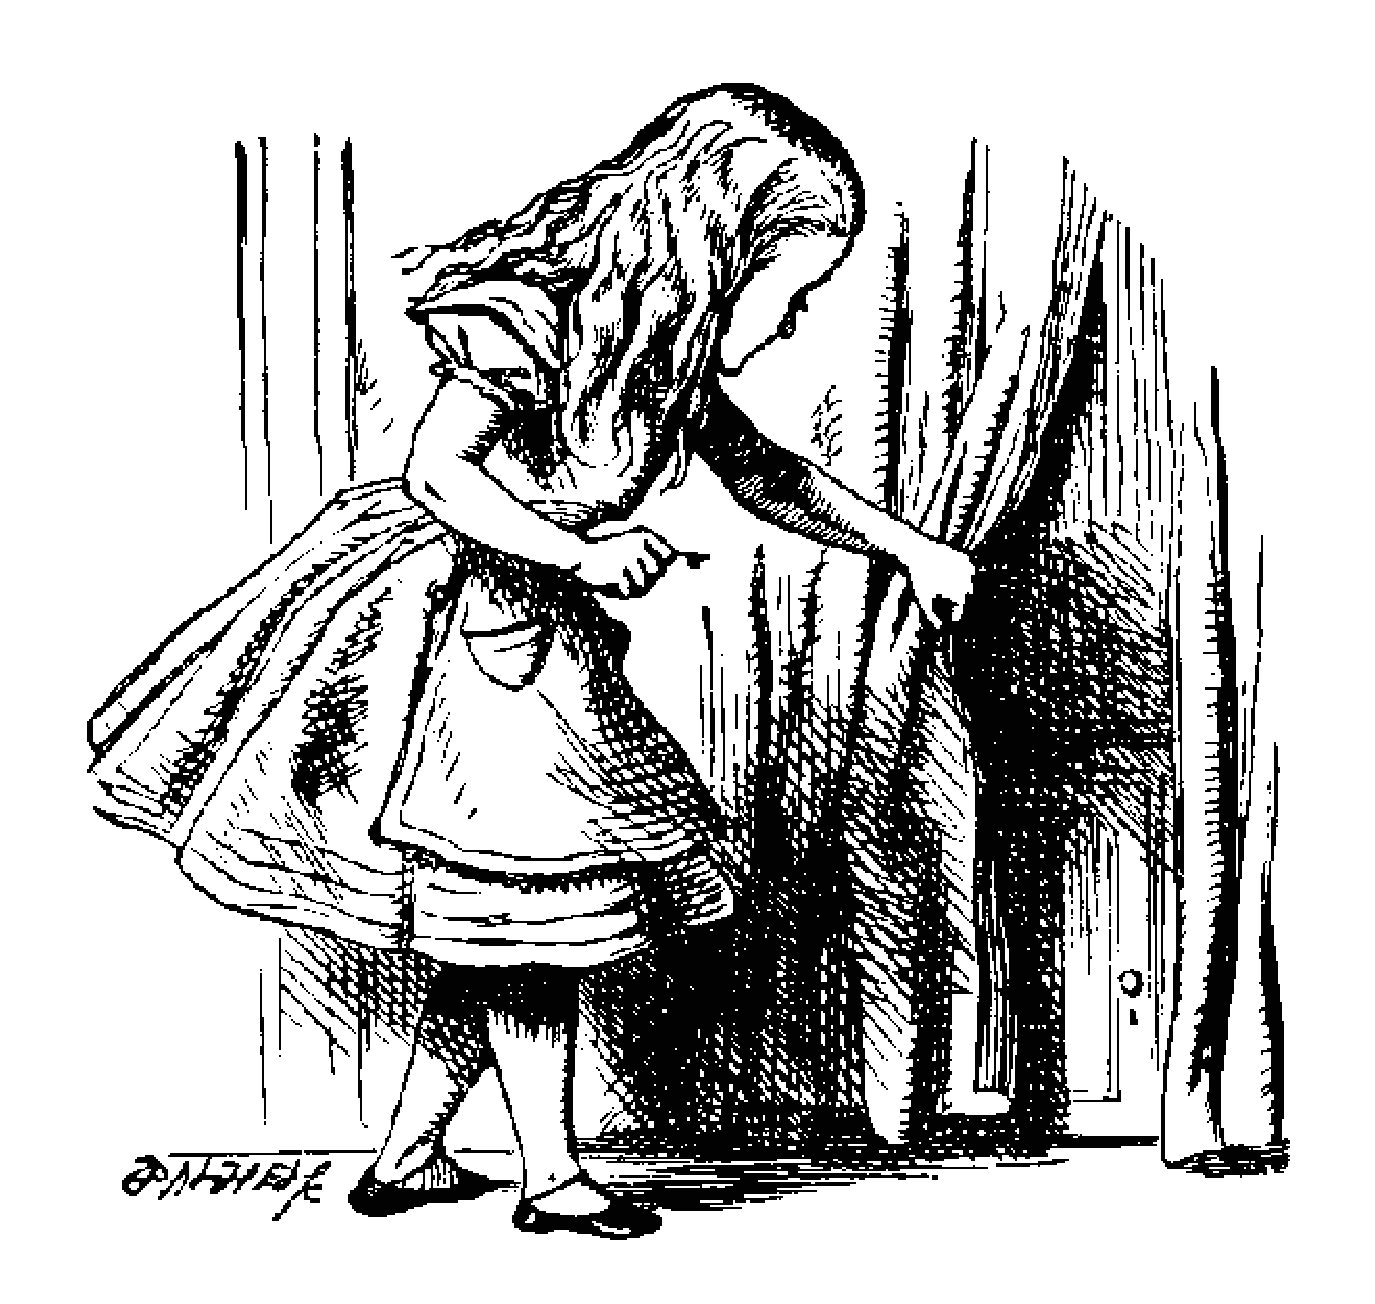
\includegraphics[width=7cm]{figures/alice}
\end{center}
\caption{Behind it was a little door}
\label{fig:alice}
\end{figure}

This is an example of how to reference an inlcuded figure (see Figure \ref{fig:alice}).

%==============================================================================
\section{Reflections}
\label{sec:reflections}

% Several sections that reflect on your experiences during the team project. Each section should discuss one theme, characterised by incidents or events that occurred during the team course of the project from which you learned (approximately 12-15 pages).

%==============================================================================
\section{Conclusions}
\label{sec:conclusions}
% A conclusion that draws general and wider lessons from the case study (approximately 1-2 pages)

Explain the wider lessons that you learned about software engineering,
based on the specific issues discussed in previous sections.  Reflect
on the extent to which these lessons could be generalised to other
types of software project.  Relate the wider lessons to others
reported in case studies in the software engineering literature.

%==============================================================================
\bibliographystyle{plain}
\bibliography{dissertation}
\end{document}
